\part{\txt{概要}{Overview}}
\label{part:outline}

\chapter{\txt{はじめに}{Preface}}

\ifjp%>>>>>>>>>>>>>>>>>>>>>>>>>>>>>>>>>>>>>>>>>>>>>>>>>>>>>>>>>>>>>>>>>>>
	本書は東北大学電気通信研究所で開発された関数型プログラミング言語
\smlsharp{}の公式ドキュメントです.
	\smlsharp{}の概要,プログラミングチュートリアル,参照マニュアル,
ツールなどの情報を含む総合ドキュメントを意図しています.
	関数型言語に慣れた人はもちろん,これからプログラミングを始めようと
する人にも,\smlsharp{}言語を使って高度なプログラミングを書き始めるために
十分な情報を提供します.
	特に,第\ref{part:tutorial}部のチュートリアルは,関数型言語の基
本的な考え方やMLプログラミングの基礎を含んでおり,ML言語の手軽な教科書と
しても使用できます.
	ML言語をより本格的に学ぶには,Standard MLの教科書
\cite{ohori00sml}をご参照ください.
  
	\smlsharp{}は,これら教科書で書かれたStandard MLと後方互換性のあ
る言語です.
	ネイティブコードコンパイラですが,対話型プログラミングもサポート
しており,だれでも手軽にMLプログラミングを楽しむことができます.
	さらに,\smlsharp{}が実現しているC言語とのシームレスな連携などの
機能は,高度で信頼性の要求される本格的な実用的システムの開発にも威力を
発揮すると信じています. 
  
	本ドキュメントを参考に,\smlsharp{}プログラミングをお楽しみくだ
さい. 
	不明な点や要望等は著者にご連絡ください.
\else%%%%%%%%%%%%%%%%%%%%%%%%%%%%%%%%%%%%%%%%%%%%%%%%%%%%%%%%%%%%%%%%%%%%
	This is the official document of \smlsharp{}, a programming
language developed at Research Institute of Electrical Communication,
Tohoku University.
	This document intends to provide comprehensive information on
\smlsharp{}, covering a user's guide, tutorials on ML and \smlsharp{}
programming, and a reference manual.
	This \version{} version only contains an overview of \smlsharp{}
and tutorials on ML and \smlsharp{} programming, which would be
sufficient for beginners who want to start writing ML programs and
for experienced ML programmer who would like to try out or switch to
\smlsharp{}.

	Send comments and questions to the authors.
\fi%%%%<<<<<<<<<<<<<<<<<<<<<<<<<<<<<<<<<<<<<<<<<<<<<<<<<<<<<<<<<<<<<<<<<<

\begin{flushright}
\txt{
2014年3月\\
東北大学電気通信研究所\\
\authors
}
{
March, 2014\\
RIEC, Tohoku University\\
\authors
}
\end{flushright}

\chapter{\txt{本書の使い方}{How to read this document}}

\ifjp%>>>>>>>>>>>>>>>>>>>>>>>>>>>>>>>>>>>>>>>>>>>>>>>>>>>>>>>>>>>>>>>>>>>
    この文書の第\ref{part:outline}部の概要と第\ref{part:tutorial}部のチュー
トリアルはMLプログラミングの基礎から\smlsharp{}が提供する高度の機能まで
を習得できる構造になっています.
	先頭から順に一気にお読みになることをおすすめします.
	お急ぎの方は,以下のページにお探しの情報があるかもしれません.
\begin{itemize}
\item {\bf \smlsharp{}の名前について:}
第\ref{sec:smlsharpHistory}節.
\item {\bf インストール方法:}
第\ref{sec:tutorialInstall}節.
\item {\bf {\tt smlsgarp}コマンドの起動モードと起動パラメタ:}
第\ref{sec:tutorialSmlsharpParameter}節.
\item {\bf \smlsharp{}開発チームと連絡先情報:} 第\ref{sec:smlsharpTeam}節.
\item {\bf \smlsharp{}ホームページ:}
\url{http://www.pllab.riec.tohoku.ac.jp/smlsharp/ja/}
\item {\bf \smlsharp{} Documnet in English:}
\url{http://www.pllab.riec.tohoku.ac.jp/smlsharp/docs/1.0/en/manual.xhtml}
\end{itemize}   

本書に関して,以下の点をご了承ください.
\begin{itemize}
\item 
	現在の第\version{}版のドキュメントはまだ未完成のドラフトです.
	特に,参照マニュアルは含まれず,MLプログラミングのチュートリ
アルも一部未完成です.

\item 随時頻繁に修正を行います.
	そのため,本文書の配布は当面xhtml形式のみとします.
	近い将来,より完成した版のPDFでの配布を検討中です.
\item
	修正・執筆にあたっては,twitterなどでの\smlsharp{}や本書へのコメントな
ども,本書の改善の参考にさせて頂いております.
	個々に言及いたしませんが,本書をご覧頂きコメントをお寄せ頂いた
方々に感謝いたします. 

\item この文書は,LaTeXとLaTeXMLを用いて作成しています.
FirefoxなどのMathMLのレンダリングが可能なブラウザでご覧ください.

\item LaTeXMLは日本語化がなされていないようです.
	本文書は{\tt jbook}クラスで書いていますが,LateXMLのpackageに
jbook用が用意されていないため,{\tt book.cls.ltxml}を
{\tt jbook.cls.ltxml}にコピーし使用しています.
	(LateXMLの日本語クラスパッケージをご存知の方はお教えください.)
\end{itemize}
\else%%%%%%%%%%%%%%%%%%%%%%%%%%%%%%%%%%%%%%%%%%%%%%%%%%%%%%%%%%%%%%%%%%%%

	The tutorials in parts~\ref{part:outline} and
\ref{part:tutorial} are structured in such a way that the reader can
learn from ML programming basics to advanced programming features
provided by \smlsharp{}.
	We recommend to read through these parts quickly in the order
they are presented.

	If you are in a harry, you may find the desired information in
one of the following pages.
\begin{itemize}
\item {\bf How to install \smlsharp{}}: Section \ref{sec:tutorialInstall}.
\item {\bf {\tt smlsharp} command parameters}: Section \ref{sec:tutorialSmlsharpParameter}.
\item {\bf \smlsharp{} development team and contact information}: 
Section \ref{sec:smlsharpTeam}.
\item {\bf On the name of \smlsharp{}}: Section \ref{sec:smlsharpHistory} (History of \smlsharp).
\item {\bf \smlsharp{} web page}: 
\url{http://www.pllab.riec.tohoku.ac.jp/smlsharp/}
\item {\bf \smlsharp{} Documnet in Japanese (プログラミング言語\smlsharp{}解説)}:
\url{http://www.pllab.riec.tohoku.ac.jp/smlsharp/docs/1.0/ja/manual.xhtml}
\end{itemize}

In reading this document, please note the following.
\begin{itemize}
\item 
	This \version{} version is an incomplete draft; it does not
contain the reference manual and the ML programming tutorial is
incomplete.

\item 
	This document is frequently revised and updated.
	For this reason, the currently version is distributed only on
this web server.
	In near future, we plan to include a more complete version of
this document (both in PDF and XHTML format) in the \smlsharp{}
distribution.

\item
	We appreciate those who give us comments on \smlsharp{} and
this document through some communication tools including Twitter.
	We have reflect all of them to the latest version of this
document.

\item 
	This document is written in LaTeX and processed with LaTeXML.
	It is best viewed with a MathML-capable browser such as {\bf Firefox}.
\end{itemize}
\fi%%%%<<<<<<<<<<<<<<<<<<<<<<<<<<<<<<<<<<<<<<<<<<<<<<<<<<<<<<<<<<<<<<<<<<

\chapter{\txt{\smlsharp{}使用上の注意}{Important notes on \smlsharp{}}}

\ifjp%>>>>>>>>>>>>>>>>>>>>>>>>>>>>>>>>>>>>>>>>>>>>>>>>>>>>>>>>>>>>>>>>>>>

\smlsharp{}\version{}版を使用する上で注意すべき点を列挙します.
\begin{enumerate}
\item
%%%%%%%%%%%%%%%%%%ToDo: functorの型引数
\end{enumerate}
\else%%%%%%%%%%%%%%%%%%%%%%%%%%%%%%%%%%%%%%%%%%%%%%%%%%%%%%%%%%%%%%%%%%%%

Here, we list the issues you should aware of in using \smlsharp{}
version~\version{}.
\begin{enumerate}
\item
%%%%%%%%%%%%%%%%%%ToDo: functorの型引数
\end{enumerate}
\fi%%%%<<<<<<<<<<<<<<<<<<<<<<<<<<<<<<<<<<<<<<<<<<<<<<<<<<<<<<<<<<<<<<<<<<

% \tableofcontents
% \mainmatter


\chapter{\txt{\smlsharp{}の概要}{Overview of \smlsharp{}}}
\label{chap:intro}

\ifjp%>>>>>>>>>>>>>>>>>>>>>>>>>>>>>>>>>>>>>>>>>>>>>>>>>>>>>>>>>>>>>>>>>>>
本章では\smlsharp{}言語の概要を説明します.
\else%%%%%%%%%%%%%%%%%%%%%%%%%%%%%%%%%%%%%%%%%%%%%%%%%%%%%%%%%%%%%%%%%%%%
This chapter outlines the \smlsharp{} language and the compiler.
\fi%%%%<<<<<<<<<<<<<<<<<<<<<<<<<<<<<<<<<<<<<<<<<<<<<<<<<<<<<<<<<<<<<<<<<<

\section{\txt{\smlsharp{}とは?}{What is \smlsharp{}?}}
\label{sec:whatIsSmlsharp}

\ifjp%>>>>>>>>>>>>>>>>>>>>>>>>>>>>>>>>>>>>>>>>>>>>>>>>>>>>>>>>>>>>>>>>>>>
\smlsharp{}は,以下のような特徴をもったML系関数型プログラミング言語です.
\begin{enumerate}
\item {\bf Standard MLとの後方互換性.}
	\smlsharp{}は,ML系言語の標準の厳密な仕様であるStandard MLとの
後方互換性を持っています.
	Standard MLの形式的な仕様\cite{sml}を満たすすべての
プログラムをコンパイルできます.

\item {\bf レコード多相性.}
	レコード多相性\cite{ohor95toplas}は,オブジェクトやデータベース
のタプルなどに現れるラベル付きレコードをML言語に完全に統合するために必要
な型システムの機能です.
	\smlsharp{}は,この機能を完全にサポートしています.

\item {\bf SQLのシームレスな統合.}
	SQLはデータベースの標準問い合わせ言語であり,データベースを利用
するプログラムで必ず必要となる機能です.
	\smlsharp{}は,SQLの一部の機能をライブラリとして提供するのでは
なく,SQLクエリそのものを多相型をもつ第一級の式として統合しています.
	この機能により,複雑なプログラムデータベース操作を,MLプログラム
の中で直接プログラムすることができます.
	
\item {\bf C言語との直接連携.}
	システムプログラミングを含む種々のOSの機能の利用にはC言語で記述
されたライブラリへのアクセスが必要となります.
	\smlsharp{}では,名前を外部名宣言するだけで,C言語で書かれCコン
パイラでコンパイルされた関数を呼び出すことができます.

\item {\bf マルチコアCPU上のネイティブスレッドのサポート.}
	\smlsharp{}の並行かつオブジェクトを動かさないGCの機能により,
C言語との連携機能を使い,OSのスレッドライブラリを直接呼び出すことができ
ます.
	従って,OSがマルチコアCPU上での並列実行をサポートしさえすれば,
スレッドを使った高水準なMLプログラムを書き,マルチコアCPU上で効率良く実
効することができます.

\item {\bf 分割コンパイルとリンク.}
	\smlsharp{}は,従来のインクリメンタルなコンパイルではない,真の分
割コンパイルを実現しています.
	各モジュールのインターフェイスの確定後は,各モジュールを独立に開
発しコンパイルやテストできます.
	さらに,\smlsharp{}コンパイラは,分割コンパイルの対象となる各ソー
スコードを,システム標準のオブジェクトファイル(例えばLinuxならば
ELFフォーマット)にコンパイルし,システムのリンカーでCのライブラリなどと
ともにリンクします.
	この機能により,Standard MLだけでなくC言語やSQLなどをも使う
大規模プログラムを安全かつ効率的に開発することができます.

\end{enumerate}

	\smlsharp{}コンパイラおよび実行時処理系は,東北大学電気通信研究
所大堀研究室で開発され,東北大学が著作権保有するオープンソースソフトウェ
アです.
	BSDスタイルの\smlsharp{}ライセンス(\ref{sec:smlsharpLicence}節参照)に
よって公開されており,だれでも自由に利用することができます.
	このライセンスは,二次著作物(つまりコンパイラで作成されたシステ
ムなど)に関する制限の少ないフリーソフトウェアライセンスであり,企業の商
品開発にも安心して使用できます.

\else%%%%%%%%%%%%%%%%%%%%%%%%%%%%%%%%%%%%%%%%%%%%%%%%%%%%%%%%%%%%%%%%%%%%
	\smlsharp{} is a new programming language in the ML-family,
having the following features.
\begin{enumerate}
\item {\bf Downward compatibility with Standard ML.}
	\smlsharp{} can compile all programs that conform to the
definition of the Standard ML\cite{sml}.

\item {\bf Record polymorphism.}
	\smlsharp{} supports record polymorphism \cite{ohor95toplas}.
	In \smlsharp{} , field selection operators {\bf\tt \#\nonterm{label}}
and record patterns {\bf\tt \{\nonterm{field-pat},...\}} are fully
polymorphic.
	This feature is essential in modular development of programs
manipulating records, and is the key to extend ML with SQL.

\item {\bf Seamless integration of SQL.}
	\smlsharp{} seamlessly integrates (currently a subset of) SQL.
	Instead of providing built-in primitives to access
database servers, \smlsharp{} integrate SQL expressions themselves as
polymorphically-typed first-class citizens.
	This allows the programmer to directly access databases in
your polymorphic ML code.

\item {\bf Direct interface to C.}
	\smlsharp{} programs can directly call C functions of your own
coding or in system libraries.
	The programmer need only declare their names and types, without
writing mysterious ``stubs'' or conversion functions. 
	The \smlsharp{} generates external references to C functions,
which are resolved and linked by the system linker.
	Both static and dynamic linking are supported.

\item {\bf Separate compilation and linking.}
	\smlsharp{} supports true separate compilation and linking.
	By writing an interface file, each source file is compiled
separately into an object file in the standard system format (e.g.\ ELF
format.)
	The separately compiled object files are then linked together
possibly with C functions and libraries into an executable program.

\item {\bf Multithread support for multicore CPUs.}
	The non-moving GC \cite{ueno11icfp} and direct C interface allow
\smlsharp{} code to directly call POSIX thread library.
	As far as the OS thread library support a multicore CPU,
\smlsharp{} program automatically obtains multithread capability for
multicore CPUs.
	With the non-moving fully concurrent GC we have just developed, 
concurrent threads run efficiently on a multicore CPU.

\end{enumerate}

	The \smlsharp{} compiler and its runtime system are developed at
Research Institute of Electrical Communication,  Tohoku University.
	They are open-source software distributed with a BSD-style
\smlsharp{} license (\ref{sec:smlsharpLicence}).
\fi%%%%<<<<<<<<<<<<<<<<<<<<<<<<<<<<<<<<<<<<<<<<<<<<<<<<<<<<<<<<<<<<<<<<<<

\section{\txt{\smlsharp{}の歴史}{History of \smlsharp{}}}
\label{sec:smlsharpHistory}

\ifjp%>>>>>>>>>>>>>>>>>>>>>>>>>>>>>>>>>>>>>>>>>>>>>>>>>>>>>>>>>>>>>>>>>>>
	1993年,沖電気工業(株)関西総合研究所にて,大堀により,Standard
ML of New Jerseyコンパイラに多相型レコード演算を加え拡張したプロトタイプ
{\bf SML\# of Kansai}が開発されました.
	その時の\smlsharp{}のtypesメーリングリストへのアナウンスは,今で
もインターネット上に記録されています
(
\url{http://www.funet.fi/pub/languages/ml/sml%23/description}
).

	{\bf SML\# of Kansai}の名前は,このコンパイラにて初めて多相型が与えら
れたレコード演算子"{\bf \code{\#}}"を象徴するものです.
	このコンパイラは,1996年ACM TOPLASに出版されたコード多相性に関する論文
\cite{ohor95toplas}で,{\bf \smlsharp{}}の名前で紹介されています.

	その後,より完全な\smlsharp{}コンパイラの開発の努
力が継続されました.

	2003年に,北陸先端科学技術大学院大学にて,文部科学省リーディング
プロジェクトe-Society基盤ソフトウェアの総合開発「高い生産性をもつ高信頼
ソフトウエア作成技術の開発」
(領域代表者:片山卓也)
の一つの課題
「プログラムの自動解析に基づく高信頼ソフトウェアシステム構築技術」(2003年―2008年,究代表者:大堀 淳)
(
\url{http://www.tkl.iis.u-tokyo.ac.jp/e-society/index.html}
)
として,
次世代ML系関数型言語\smlsharp{}をスクラッチから開発するプロジェクトを開始しました.

2006年4月,プロジェクトは,大堀とともに東北大学電気通信研究所に移り開発
を継続しています.

2008年のe-Societyプロジェクト終了後も,東北大学電気通信研究所大堀研究室
にて,\smlsharp{}の研究開発を続けています.

\else%%%%%%%%%%%%%%%%%%%%%%%%%%%%%%%%%%%%%%%%%%%%%%%%%%%%%%%%%%%%%%%%%%%%

	In 1993, Atsushi Ohori extended the Standard ML of New Jersey
compiler at Kansai Laboratory of Oki Electric, and named the
experimental prototype SML\# of Kansai.
	The Internet still remembers my old posting of \smlsharp{} to
the types mailing list 
(\url{http://www.funet.fi/pub/languages/ml/sml%23/description}).

	The name SML\# of Kansai symbolizes the field selector {\bf\tt
\#\nonterm{label}}, which was given a polymorphic type for the first
time by this compiler.
	This compiler was reported in the ACM TOPLAS article on record
polymorphism \cite{ohor95toplas} as {\bf \smlsharp{}}.

	To support not only record polymorphism but also
interoperability and other practically important features, we decided 
to develop a new SML-style language from scratch, and in 2003, we
started the \smlsharp{} compiler project at Japan Advanced Institute of 
Science and Technology as a part of the e-Society project 
(
\url{http://www.tkl.iis.u-tokyo.ac.jp/e-society/index.html}
).
funded by the Japan ministry of science, education and technologies

	In 2006, the project moved to Tohoku University.
\fi%%%%<<<<<<<<<<<<<<<<<<<<<<<<<<<<<<<<<<<<<<<<<<<<<<<<<<<<<<<<<<<<<<<<<<

\section{
\txt{\smlsharp{}開発チームと連絡先情報}
{\smlsharp{} Development Team and Contact Information}
}
\label{sec:smlsharpTeam}

\ifjp%>>>>>>>>>>>>>>>>>>>>>>>>>>>>>>>>>>>>>>>>>>>>>>>>>>>>>>>>>>>>>>>>>>>
	現在(2014年3月)\smlsharp{}は,
\begin{itemize}
\item 
大堀 淳(東北大学電気通信研究所)
\item 
上野雄大(東北大学電気通信研究所)
\end{itemize}
の2名が,大学院大学院情報科学研究科の大堀研究室に所属の大学院生の協力の
下,開発を行なっています.

	\smlsharp{}のこれまでの主な開発者は以下の通りです.
	(敬称は略させていただいています.
	所属は\smlsharp{}の開発に携わった時のものです.)
\begin{itemize}
\item 大堀 淳(北陸先端科学技術大学院大学情報科学研究科,東北大学電気通信研究所)
\item 大和谷 潔(算譜工房)
\item Nguyen Huu Duc(北陸先端科学技術大学院大学情報科学研究科,東北大学電気通信研究所)
\item Liu Bochao(北陸先端科学技術大学院大学情報科学研究科,東北大学電気通信研究所)
\item 纓坂 智(北陸先端科学技術大学院大学情報科学研究科)
\item 上野雄大(北陸先端科学技術大学院大学情報科学研究科,東北大学電気通信研究所)
\end{itemize}

	東北大学電気通信研究所では,\smlsharp{}に関する情報共有の目的で
以下のwebサイトやメーリングリストを管理しています.
\begin{itemize}
\item \smlsharp{}ホームページ.
\url{http://www.pllab.riec.tohoku.ac.jp/smlsharp/ja/}
コンパイラや本書を含む文書の最新版などもここからダウンロードできます.

\item \smlsharp{}メーリングリスト
{\tt smlsharp@ml.riec.tohoku.ac.jp}.
\smlsharp{}に関する一般的な議論や情報交換のためのメーリングリストです.
使用言語は日本語または英語です.投稿は購読者のみ行うことができ,投稿され
た全てのメールはWeb上に公開されます.\\
%%%%%%%%%%%%%%%%%%ToDo: 参加方法
%参加方法:\url{http://www.pllab.riec.tohoku.ac.jp/mailman/listinfo.cgi/smlsharp-list?language=ja}\\
%アーカイブ:\url{http://www.pllab.riec.tohoku.ac.jp/pipermail/smlsharp-list/}

\item Twitterアカウント {\tt @smlsharp}.
\smlsharp{}に関する最新情報をツイートします.

\item \smlsharp{}開発者への連絡メールアドレス.
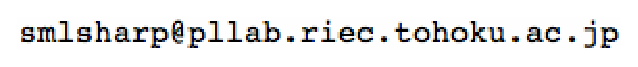
\epsfig{file=smlsharp-list.eps,width=0.4\textwidth}
共同研究の提案や各種問い合わせなどにご利用ください.
\end{itemize}
\else%%%%%%%%%%%%%%%%%%%%%%%%%%%%%%%%%%%%%%%%%%%%%%%%%%%%%%%%%%%%%%%%%%%%
	At present (March 2014), \smlsharp{} is being developed by
\begin{itemize}
\item 
Atsushi Ohori(RIEC, Tohoku University)
\item 
Katsuhiro Ueno (RIEC, Tohoku University)
\end{itemize}
with help of graduate students.

	The past \smlsharp{} development team members include (with the
affiliation at the time of development):
\begin{itemize}
\item Atsushi Ohori (School of Information Science, JAIST; RIEC, Tohoku University)
\item Kiyoshi Yamatodani (Sanpukoubou Inc)
\item Nguyen Huu Duc (School of Information Science, JAIST; RIEC, Tohoku University)
\item Liu Bochao (School of Information Science, JAIST; RIEC, Tohoku University)
\item Satoshi Osaka (School of Information Science, JAIST)
\item Katsuhiro Ueno (School of Information Science, JAIST; RIEC, Tohoku University)
\end{itemize}

	Contact information regarding \smlsharp{}:
\begin{itemize}
\item \smlsharp{} home page:
\url{http://www.pllab.riec.tohoku.ac.jp/smlsharp/ja/}

\item \smlsharp{} mailing list:
{\tt smlsharp-list@pllab.riec.tohoku.ac.jp}

	This list is for general discussion on \smlsharp{}.
	We use Japanese and English in discussion.
	To post a message, you need to subscribe to this list.
	All the messages are made available on the Web.

%%%%%%%%%%%%%%%%%%ToDo: 参加方法
%How to subscribe:\url{http://www.pllab.riec.tohoku.ac.jp/mailman/listinfo.cgi/smlsharp-list?language=ja}\\
%Mail archive:\url{http://www.pllab.riec.tohoku.ac.jp/pipermail/smlsharp-list/}

\item \smlsharp{} twitter account:
{\tt @smlsharp}

	We tweet the latest information about \smlsharp{} on this account.

\item Email address of the \smlsharp{} development team :
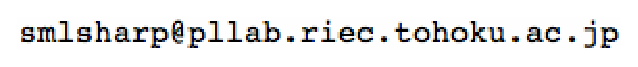
\epsfig{file=smlsharp-list.eps,width=0.4\textwidth}

Send your questions, requests and comments to the development team.
\end{itemize}
\fi%%%%<<<<<<<<<<<<<<<<<<<<<<<<<<<<<<<<<<<<<<<<<<<<<<<<<<<<<<<<<<<<<<<<<<

\section{\txt{謝辞}{Acknowledgments}}
\label{sec:acknowledgements}
	
\ifjp%>>>>>>>>>>>>>>>>>>>>>>>>>>>>>>>>>>>>>>>>>>>>>>>>>>>>>>>>>>>>>>>>>>>
	2003年にスタートした\smlsharp{}開発の過程では,以下を含む色々な
ご指導やご協力を頂きました.
	ここに謝意を表します.
\else%%%%%%%%%%%%%%%%%%%%%%%%%%%%%%%%%%%%%%%%%%%%%%%%%%%%%%%%%%%%%%%%%%%%
	From its start in 2003, we have benefited from many pepples and
ogranizations.
\fi%%%%<<<<<<<<<<<<<<<<<<<<<<<<<<<<<<<<<<<<<<<<<<<<<<<<<<<<<<<<<<<<<<<<<<
	
\subsection{\txt{プロジェクトファンディング}{Project funding}}

\ifjp%>>>>>>>>>>>>>>>>>>>>>>>>>>>>>>>>>>>>>>>>>>>>>>>>>>>>>>>>>>>>>>>>>>>
	\smlsharp{}言語の研究開発は,2003年から5年間の文部科学省リーディ
ングプロジェクトe-Society基盤ソフトウェアの総合開発「高い生産性をもつ高
信頼ソフトウェア作成技術の開発」
(\url{http://www.tkl.iis.u-tokyo.ac.jp/e-society/index.html)}
の一つの課題
「プログラムの自動解析に基づく高信頼ソフトウェアシステム構築技術」(究代
表者:大堀 淳)としてスタートをきることができました.
	このプロジェクトの主要な目標が\smlsharp{}言語コンパイラの開発で
した.
	\smlsharp{}は開発ソースの総量が\smlsharpSize{}行を超える大規模シ
ステムです.
	このプロジェクトの支援がなければ,\smlsharp{}の開発は困難であっ
たと思われます.
	文部科学省,e-Societyの領域代表の片山卓也先生,および関係各位に
深謝いたします.
\else%%%%%%%%%%%%%%%%%%%%%%%%%%%%%%%%%%%%%%%%%%%%%%%%%%%%%%%%%%%%%%%%%%%%
	\smlsharp{} development was started as a part of the 5 year
project 
``e-Society leading project: highly productive reliable software
development technologies (Project Director: Professor Takuya Katayama)'' 
under the title
``
reliable software development technology based on automatic program analysis
(chief investigator: Atsushi Ohori)
''
(\url{http://www.tkl.iis.u-tokyo.ac.jp/e-society/index.html})
sponsored by the Japan ministry of science, education and technologies.
\fi%%%%<<<<<<<<<<<<<<<<<<<<<<<<<<<<<<<<<<<<<<<<<<<<<<<<<<<<<<<<<<<<<<<<<<

\subsection{
\txt{\smlsharp{}が使用しているソフトウエア}
    {Third-party code and software tool used in \smlsharp{} development}
}

\ifjp%>>>>>>>>>>>>>>>>>>>>>>>>>>>>>>>>>>>>>>>>>>>>>>>>>>>>>>>>>>>>>>>>>>>
	\smlsharp{}言語は,第1.0版以降は,\smlsharp{}自身でコンパ
イルし開発を行なっていますが,それ以前は,Standard ML of New Jerseyおよ
びMLtonのStandard MLコンパイラを使って開発を行いました.

	\smlsharp{}は前節(\ref{sec:smlsharpTeam})の開発チー
ムによって開発されたソフトウェアです.
	ソースコードの殆どをスクラッチから開発しましたが,一部に以下のコー
ドを利用しています.

\begin{center}
\begin{tabular}{|l|l|l|}
\hline
内容 & \smlsharp{}ソース上の位置 & ソース
\\\hline
ML-Yacc & src/ml-yacc  & Standard ML of New Jersey 110.73
\\\hline
ML-Lex & src/ml-lex  & Standard ML of New Jersey 110.73
\\\hline
SML/NJ Library & src/smlnj-lib &  Standard ML of New Jersey 110.73
\\\hline
TextIO,
BinIO,
OS,
Timer
&
src/smlnj
&
Standard ML of New Jersey 110.73
\\\hline
浮動小数点/
文字列変換関数
&
src/runtime/netlib
&
the Netlib
\\\hline
SMLFormatの
SML文法定義
&
src/smlformat/generator/main/
&
Standard ML of New Jersey 110.73
\\\hline
\end{tabular}
\end{center}

	これらソースは,いずれも\smlsharp{}ライセンスと整合性あるライセ
ンスで配布されているオープンソースソフトウェアです.
	「\smlsharp{}ソース上の位置」にそれぞれのライセンスが添付されて
います.
\else%%%%%%%%%%%%%%%%%%%%%%%%%%%%%%%%%%%%%%%%%%%%%%%%%%%%%%%%%%%%%%%%%%%%

	Since version 1.0 had completed, \smlsharp{} has been
developed by the \smlsharp{} compiler itself.
	Before the \version{} version, we had used Standard ML of New
Jersey compiler for development and MLTon compiler for building
distributions.

	The \smlsharp{} compiler is a software developed by the
\smlsharp{} development team (\ref{sec:smlsharpTeam}).
	We have wrote most of the code of \smlsharp{} compiler from
scratch, except for the following code: 

\begin{center}
\begin{tabular}{|c|c|c|}
\hline
contents & location in \smlsharp{} distribution & source code
\\\hline
ML-Yacc & src/ml-yacc  & Standard ML of New Jersey 110.73
\\\hline
ML-Lex & src/ml-lex  & Standard ML of New Jersey 110.73
\\\hline
SML/NJ Library & src/smlnj-lib &  Standard ML of New Jersey 110.73
\\\hline
{\tt TextIO},
{\tt BinIO},
{\tt OS},
{\tt Timer}
structures
&
src/smlnj
&
Standard ML of New Jersey 110.73
\\\hline
floating point-string conversion
(dtoa.c)
&
src/runtime/netlib
&
the Netlib
\\\hline
SML grammar definition used 
in SMLFormat tool
&
src/smlformat/generator/main/
&
Standard ML of New Jersey 110.73
\\\hline
\end{tabular}
\end{center}

	All of the above are open-source software that are compatible
with \smlsharp{} license.
	The \smlsharp{} source distribution includes the license of each
of them at the ``location in \smlsharp{} distribution'' show above.
\fi%%%%<<<<<<<<<<<<<<<<<<<<<<<<<<<<<<<<<<<<<<<<<<<<<<<<<<<<<<<<<<<<<<<<<<

\subsection{\txt{研究開発協力者}{Collaborators}}

\ifjp%>>>>>>>>>>>>>>>>>>>>>>>>>>>>>>>>>>>>>>>>>>>>>>>>>>>>>>>>>>>>>>>>>>>
	\smlsharp{}言語の開発にあたっては,多くの人々からの指導を受けま
した.
	過去現在の開発チーム(第(\ref{sec:smlsharpTeam})節)以外で特に
貢献のあった方々は以下の通りです.
\begin{itemize}
\item 篠埜功氏.
大堀と共に,関数フュージョン機能を持つ新たしいインラインの理論および
その実験的な実装を行いました.
	この機能は実験的な実装がありますが,まだ十分な完成度が得られてお
らず\smlsharp{}\version{}版に組み込まれていませんが,将来取り入れたいと
考えています.
\item 大友聡顕氏.
	大堀,上野と共に,オブジェクトを動かさないGCの研究開発に携わり,
初期の実験的な実装を行い,この方式が有望であることを確認しました.
	この成果は,現在のオブジェクトを動かさないGCの方式の開発と実装の
契機となったものです.
\end{itemize}
	これらの方々以外にも,\smlsharp{}は,大堀等との共同で行なった様々
な型理論やコンパイル方式の基礎研究を基に設計されています.
	現在の\smlsharp{}言語に直接生かされている出版された基礎研究成果
には以下のものが含まれます.
\begin{itemize}
\item レコード多相性の理論\cite{ohor92popl,ohor95toplas}.
\item データベースの型推論\cite{ohor88lfp}.
\item データベース言語(Machiavelli)\cite{ohor89sigmod,bune96tods}.
\item ランク1多相性の型理論\cite{ohor99icfp}.
\item MLのunboxed意味論\cite{ohor97unbox}.
\item MLにおける自然なデータ表現\cite{nguyen06ppdp}.
\item オブジェクトを動かさないGC\cite{ueno11icfp}.
\item 軽量の関数融合\cite{ohor07popl}.
\end{itemize}
	それ以外にも多くの共同研究者から色々な機会に示唆や助言を頂いてお
り,それらは1989年にまで遡りますが,それらの方々の列挙は割愛させてい
ただきます.
\else%%%%%%%%%%%%%%%%%%%%%%%%%%%%%%%%%%%%%%%%%%%%%%%%%%%%%%%%%%%%%%%%%%%%

	Many people have contributed to research and development of
\smlsharp{}.
	In addition to the development team (Section
\ref{sec:smlsharpTeam}), the following people directly contributed to 
\smlsharp{} research.
\begin{itemize}
\item Isao Sasano.
With Atsushi Ohori, he investigated 
``Lightweight fusion by fixed point promotion'' and 
developed an experimental inlining module that performs lightweight
fusion.
	This feature is experimental and has not yet been integrated in
\smlsharp{} compiler, but we plan to adopt this method in a future
version.
\item Toshihiko Otomo.
	With Atsushi Ohori and Katsuhiro Ueno, he investigated the
possibility of non-moving collector and showed an initial experimental
result indicating that a non-moving GC is viable in functional
languages.
\end{itemize}
	Many other people helped us through collaborative research with
Atsushi Ohori and others to develop type-theory and compilation methods
that underlie \smlsharp{} compiler.
	\smlsharp{} compiler is directly based on the
following research results, some of them were collaboratively done.
\begin{itemize}
\item record polymorphism \cite{ohor92popl,ohor95toplas}.
\item database type inference \cite{ohor88lfp}.
\item database language (Machiavelli)\cite{ohor89sigmod,bune96tods}.
\item rank-1 polymorphism \cite{ohor99icfp}.
\item unboxed semantics of ML \cite{ohor97unbox}.
\item natural data representation for ML \cite{nguyen06ppdp}.
\item efficient non-moving GC\cite{ueno11icfp}.
\item lightweight fusion \cite{ohor07popl}.
\end{itemize}
	We have also benefited from many other researchers from 1989.
	We refrain from compiling a comprehensive list, which seems to
be impossible. 
\fi%%%%<<<<<<<<<<<<<<<<<<<<<<<<<<<<<<<<<<<<<<<<<<<<<<<<<<<<<<<<<<<<<<<<<<

\section{\txt{\smlsharp{}ライセンス}{\smlsharp{} License}}
\label{sec:smlsharpLicence}

Copyright (c) 2006 - 2014, Tohoku University.\\
All rights reserved.\\

Redistribution and use in source and binary forms, with or without
modification, are permitted provided that the following conditions are
met:

\begin{itemize}
\item 
  Redistributions of source code must retain the above copyright
  notice, this list of conditions and the following disclaimer. 
\item 
  Redistributions in binary form must reproduce the above
  copyright notice, this list of conditions and the following disclaimer
  in the documentation and/or other materials provided with the
  distribution. 
\item 
  Neither the name of Tohoku University nor the names of its
  contributors may be used to endorse or promote products derived from
  this software without specific prior written permission.  
\end{itemize}

THIS SOFTWARE IS PROVIDED BY TOHOKU UNIVERSITY AND CONTRIBUTORS "AS IS"
AND ANY EXPRESS OR IMPLIED WARRANTIES, INCLUDING, BUT NOT LIMITED TO,
THE IMPLIED WARRANTIES OF MERCHANTABILITY AND FITNESS FOR A PARTICULAR
PURPOSE ARE DISCLAIMED. IN NO EVENT SHALL TOHOKU UNIVERSITY OR
CONTRIBUTORS BE LIABLE FOR ANY DIRECT, INDIRECT, INCIDENTAL, SPECIAL,
EXEMPLARY, OR CONSEQUENTIAL DAMAGES (INCLUDING, BUT NOT LIMITED TO,
PROCUREMENT OF SUBSTITUTE GOODS OR SERVICES; LOSS OF USE, DATA, OR
PROFITS; OR BUSINESS INTERRUPTION) HOWEVER CAUSED AND ON ANY THEORY OF
LIABILITY, WHETHER IN CONTRACT, STRICT LIABILITY, OR TORT (INCLUDING
NEGLIGENCE OR OTHERWISE) ARISING IN ANY WAY OUT OF THE USE OF THIS
SOFTWARE, EVEN IF ADVISED OF THE POSSIBILITY OF SUCH DAMAGE.

\section{
\txt{\smlsharp{}第\version{}版の機能と制限}
{Limitations in \smlsharp{} version \version{}}
}
\label{sec:smlsharpLimitation}

\ifjp%>>>>>>>>>>>>>>>>>>>>>>>>>>>>>>>>>>>>>>>>>>>>>>>>>>>>>>>>>>>>>>>>>>>
	我々開発チームは第\ref{sec:whatIsSmlsharp}節でのべた機能をすべて
開発し\smlsharp{}開発開始時に目標とした機能を実現しています.
	第\version{}版にその殆どが含まれていますが,以下の制約があります.
\begin{enumerate}
\item POSIX ネイティブスレッド.
	この機能は現時点では,十分にテストされていないため,デフォルトで
はオフになっています.
	システム構築時({\tt ./configure}時)に{\tt --enable-thread}
を指定すればオンになり,コンパイラはPOSIX thread対応のコードを生成します.
	POSIX thread APIを{\tt \_import}すれば,マルチコア上でネイ
ティブスレッドが利用可能です.

\item ターゲットアーキテクチャ.
	現在の\smlsharp{}コンパイラは,32ビットのIntelアーキテクチャ
(x86, IA-32)向けのコードのみ生成可能です.
	将来,マルチターゲット化を行う予定です.
	特に,Intel系64ビットアーキテクチャ(x64またはamd64)への対応は
近い将来行う予定です.
	\smlsharp{}\version{}版はコンパイラバックエンドにLLVMを用いており,
この対応は容易と思われます.

%\item Windows版の対話型ループの制約.
%	\smlsharp{}\version{}版は,すべて一つのネイティブコードコンパイ
%ラで動いています.
%	対話型ループも,(1)ユーザ入力のコンパイル,
%(2)現在のコンパイラにリンク,
%(3)動的にロード,のサイクルによって実現されています.
%	この中で(2)のリンクをWindowsシステム上で実現するためには,シ
%ステムの制約上,これまでに作られたオブジェクトファイル毎にリンクのための
%ファイルをコマンドラインで指定する必要があります.
%	このファイル数が,対話型環境での入力に従って増えて行きます.
%	そのため,Windows上の対話型環境の連続使用は,コマンドラインの最
%大文字数によって制約されます.

\item 最適化.
	現在のバージョンには,インライニングや定数の伝播などの基本的な最
適化も十分に実装されていません.
	従って,コンパイル時間,コンパイルされたコードの実行時間もともに
十分とは言えません.
%	現在,最適化の設計開発を開始しました.
	将来の版では,他の最適化コンパイラに比肩する速度が得られると期待
しています.
\end{enumerate}
\else%%%%%%%%%%%%%%%%%%%%%%%%%%%%%%%%%%%%%%%%%%%%%%%%%%%%%%%%%%%%%%%%%%%%
	We have successfully developed all the features listed in
Section~\ref{sec:whatIsSmlsharp}, which we had initially aimed at.
	The version \version{} contains most of them, with the following 
restrictions.
\begin{enumerate}
\item {\bf POSIX Native thread support}

	This feature has not yet been well tested.
	So we set it off by default.
	To enable it, give {\tt --enable-thread} to {\tt ./configure}. 
	The compiler then generate thread-safe code.
	If you import OS thread-library through {\tt \_import}
declaration, your multithread code should run on multicore CPU.

	We have also completed development of a fully concurrent
non-moving GC.
	This has not been integrated in \version{} version.
	The GC in the \version{} version is a stop-the-world multithread
extension of the non-moving GC.
	We will replace this with a fully concurrent non-moving GC in
a future version.

\item {\bf Target Architecture.}

	The current compiler only generates x86 (or IA-32) code.
	We plan to support any other platforms, in particular amd64 (or x64),
in near future.
	Since \smlsharp{}\version{} uses LLVM as its compiler backend,
it seems to be easy for \smlsharp{} to support multiple platforms.

\item {\bf Optimization.}

	In this version, optimization is far from adequate; it does not
even implement standard ones such as inlining and constant propagation.
	So both the compilation time and the speed of generated code are
not very satisfactory.
	We have started design and development of optimizing \smlsharp{}
compiler, and hope that we will provide an optimized \smlsharp{}
compiler that is as fast as other mature compilers.

%\item {\bf Interface language.}
%
%	To support separate compilation, we have defined the interface
%language for \smlsharp{} source code.
%	This is our initial design and has a room of improvement.
%	We hope to improve the interface language based on our experience
%and other user's comments and requests.

%\item {\bf SQL integration.}
%
%	The current version only supports PostgreSQL.
%	The available SQL constructs are also limited.
%	In future version, we shall support fuller SQL syntax and
%multiple servers including MySQL.

%\item {\bf Interactive loop on Windows Systems.}
%
%	\smlsharp{} realizes interactive loop by (1) compiling the input
%to an object file, (2) linking with the currently running system to
%generate a dynamically loadable file, and then (3) dynamically loading
%the object code using {\tt dlopen}. 
%	In Windows systems, performing the linking in step 2 requires
%to specify a link information file for each of all the previous object
%files.
%	This implies that the command-line arguments to \smlsharp{}
%compiler uses in step 2 keep increasing during the interactive session,
%and will hit the limit of the command-line length. 
%	At that point, the interactive session may stall.

\end{enumerate}
\fi%%%%<<<<<<<<<<<<<<<<<<<<<<<<<<<<<<<<<<<<<<<<<<<<<<<<<<<<<<<<<<<<<<<<<<

% \section{第1章の用語解説及ぶFAQ}
% \label{sec:glossary1}
% 
% \begin{description}
% \item[BSDスタイルライセンス] 
% 二次著作物に関する制限が少ないオープンソースソフトウェアライセンスの一つ.
% 
% BSDスタイルライセンスでは,ライセンス内容をドキュメント等に表示する限り,
% ソースおよびバイナリ形式をとわず,コードの使用,変更,再配布を認めている.
% これにより,二次著作物,つまりそのソフトを利用して作成される種々の製品を,
% 自由に作成し配布や販売することができる.
% 
% 正確にな内容は英文のBSDライセンス(BSD License,Berkeley Software
% Distribution License)を参照.
% 
% 
% \item[メタ] 
% 「後に」あるいは「越えて」といった位置を表すギリシャ語.
% この接頭語を含むギリシャ語metaphsicaがアリストテレスのよって書かれた名前
% の付けられなかった本の題名の代わに使われることによって,
% 「「自然学」の後に位置する本」という意味のmetaphsicaが,
% その本の内容である「哲学,形而上学(metaphisics)」
% を意味する用語として定着した.
% それに伴い,もともとの位置の概念であったmetaに,自然学を超越する
% という意味が与えられ,種々の分野で使用されようになった.
% たとえば言語学の分野では,metaは,通常の言語の使用を分析するために用いる
% 言語として使用される.
% \end{description}
% 
% FAQ:
% \begin{itemize}
% \item 
% {[Q]} \smlsharp{}の開発に参加したいのですが?\\
% {[A]} もちろん可能です.意欲のある方はご連絡ください.一緒にプログラミング
% 言語の色々な機能を実現していきましょう.今後,研究室以外の人々とのソース
% の共有や変更の管理等の体制を整えていく予定です.
% 
% \item  
% {[Q]} 東北大学電気通信研究所でプログラミングを学ぶことができますか?\\
% {[A]} 東北大学電気通信研究所の不タッフ(教授,准教授,助教)は,学部は工学
% 部,大学院は情報科学研究科または工学研究科大学院の教員を兼務し,工学部知
% 能情報システム総合学科の学部4年生,および教員の所属する情報科学研究科お
% よび工学研究科大学院の学生を受け入れています.大堀研究室は情報科学研究科
% の教員を兼務しています.
% 
% 学部の場合は,工学部知能情報システム総合学科に,大学院なら情報科学研究科
% に入学し大堀研究室を志望すれば,我々と一緒に\smlsharp{}やその他プログラ
% ミング言語及びデータベースの研究開発を思う存分行うことができます.
% 
% \end{itemize}

